\documentclass[a4paper,11pt,twocolumn]{article}

\usepackage{aas_macros}

\usepackage[utf8]{inputenc}
\usepackage[T1]{fontenc}
\usepackage{lmodern}
%\usepackage{times}
%\usepackage[margin=2cm]{geometry}
\usepackage[a4paper]{geometry}
\usepackage{amsmath}
\usepackage{mathtools}
\usepackage{graphicx}
\usepackage{multirow}
\usepackage{multicol}
\usepackage{blindtext}
\usepackage{hyperref}
\usepackage{float}

\usepackage{pgfplotstable}
\usepackage{booktabs}
% \pgfplotsset{compat=1.18}

\usepackage[authoryear]{natbib}

\graphicspath{ {./images/} }

\usepackage[czech]{babel}
\usepackage{graphicx}
\usepackage{amsmath}
\usepackage{xspace}
\usepackage{url}
\usepackage{siunitx}
\usepackage{indentfirst}
\usepackage{subcaption}
\usepackage{caption}
\usepackage{tabularx}
\usepackage{rotating}
\usepackage{tikz}
\usepackage[labelformat=parens,labelsep=quad,skip=3pt]{caption}

\usepackage{color}
\usepackage{listings}

\definecolor{codegreen}{rgb}{0,0.6,0}
\definecolor{codegray}{rgb}{0.5,0.5,0.5}
\definecolor{codepurple}{rgb}{0.58,0,0.82}
\definecolor{backcolour}{rgb}{0.95,0.95,0.92}

\lstdefinestyle{mystyle}{
    backgroundcolor=\color{backcolour},
    commentstyle=\color{codegreen},
    keywordstyle=\color{magenta},
    numberstyle=\tiny\color{codegray},
    stringstyle=\color{codepurple},
    basicstyle=\ttfamily\footnotesize\centering,
    breaklines=true,
    captionpos=b,
    numbers=left,
    numbersep=5pt,
    showspaces=false,
    showstringspaces=false,
    showtabs=false,
    tabsize=2
}

\lstset{style=mystyle}

%\widowpenalty 10000 \clubpenalty 10000 \displaywidowpenalty 10000
\setcounter{topnumber}{3}
\setcounter{bottomnumber}{3}
\setcounter{totalnumber}{6}
\renewcommand\topfraction{0.9}
\renewcommand\bottomfraction{0.9}
\renewcommand\textfraction{0.1}
\intextsep=8mm \textfloatsep=8mm

\renewcommand{\thesection}{\arabic{section}.}
\renewcommand{\thesubsection}{\thesection\arabic{subsection}.}
\makeatletter \def\@seccntformat#1{\csname the#1\endcsname\hspace{1ex}} \makeatother


\begin{document}
    \twocolumn[
    \noindent\hrulefill
    \begin{center}
        \bigskip
        \huge Periodová analýza
        \vspace{0.2cm}
        \par \large F4191: Praktikum z astronomie 2
        \par \large Artem Gorodilov
        \vspace{0.2cm}
        \par \large 23. ~ledna 2025
        \bigskip
    \end{center}
    \noindent\hrulefill
    \bigskip
    ]

    \vskip10pt

    \section{Abstrakt}
        V této práci jsem analyzoval světelné křivky šesti neznámých objektů a také světelnou křivku hvězdy Kepler-22. Pro analýzu jsem sestrojil periodogramy pro frekvence < 10 cyklů/den a určil čtyři signifikantní frekvence, z nichž jsem získal odpovídající periody charakterizující hypotetické rekurentní změny systému. 
        
        Výpočty byly provedeny pomocí skriptu v Pythonu (viz. \citet{github}).

    \section{Úvod}
        Periodogram je nástroj používaný k analýze časových řad, například světelných křivek hvězd, za účelem identifikace periodických signálů. Princip jeho činnosti spočívá v transformaci časových dat na frekvenční doménu a měření síly variability při různých frekvencích.

        Matematicky je periodogram založen na Lomb-Scarglově metodě, která je zvláště vhodná pro nerovnoměrně vzorkované časové řady. Tato metoda odhaduje periodogram jako:
        
        \begin{equation*}
            \begin{aligned}
                P(f) = \frac{1}{2\sigma^2} \Bigg[ 
                &\frac{\left( \sum_{i} w_i (x_i - \bar{x}) \cos(2\pi f (t_i - \tau)) \right)^2}
                {\sum_{i} w_i \cos^2(2\pi f (t_i - \tau))} \\
                &+ 
                \frac{\left( \sum_{i} w_i (x_i - \bar{x}) \sin(2\pi f (t_i - \tau)) \right)^2}
                {\sum_{i} w_i \sin^2(2\pi f (t_i - \tau))} 
                \Bigg],
            \end{aligned}
        \end{equation*}

        kde $f$ je frekvence, $x_i$ jsou hodnoty dat (např. jas hvězdy), $t_i$ jsou odpovídající časy, $\sigma^2$ je rozptyl dat, $\bar{x}$ je průměr dat a $\tau$  je korekce pro fázi.
            
        Výstupem periodogramu jsou frekvence, které odpovídají dominantním periodicím v datech, například rotačním periodám hvězd nebo oběžným periodám exoplanet. Hlavní vrcholy v periodogramu představují frekvence, na kterých je variabilita nejvýraznější. Výška těchto vrcholů udává sílu variability na dané frekvenci. Významné vrcholy mají hodnoty, které výrazně převyšují úroveň šumu, jež v periodogramu funguje jako základní hladina. Šum slouží k odlišení skutečných signálů od náhodných fluktuací v datech.

        SNR (Signal-to-Noise Ratio) je poměr mezi silou signálu a úrovní šumu. V kontextu periodogramu se SNR vypočítává jako poměr výšky vrcholu (síly signálu) k průměrné nebo mediánové úrovni šumu. Matematicky lze SNR vyjádřit jako:

        \begin{equation*}
            \text{SNR} = \frac{P_{\text{peak}}}{P_{\text{noise}}},
        \end{equation*}

        kde $P_{\text{peak}}$ je hodnota výkonu na dané frekvenci (vrchol periodogramu) a $P_{\text{noise}}$ je úroveň šumu. Vysoká hodnota SNR naznačuje, že detekovaný signál je silnější než šum, a tím pádem pravděpodobně skutečný.

        FAP (False Alarm Probability) je pravděpodobnost, že detekovaný vrchol v periodogramu vznikl náhodně, vlivem šumu, a nikoli jako důsledek skutečné periodické variability. Nižší hodnota FAP znamená vyšší důvěru ve skutečnost detekovaného signálu.

    \section{Zpracování dat}
        \subsection{Data}
            Analyzoval jsem světelné křivky šesti neznámých objektů. Každá křivka byla pozorována v časovém intervalu přibližně 300 dní. 

            Pro analýzu periodického chování objektu Kepler-22 (KepID: 10593626) jsem zkombinoval tři světelné křivky získané observatoří Kepler. Vybral jsem si OBSID s následujícími daty a expozicemi:

            \begin{center}
                2009131105131, 2015-08-26, 9.73 d
                2009166043257, 2015-09-01, 33.5 d
                2009259160929, 2015-09-06, 88.98 d
                009350155506, 2015-09-09, 89.29 d
                2010078095331, 2015-09-11, 89.85 d
            \end{center}

            Celková doba pozorování byla 311.33 dní.

            Světelné křivky Keplera použité v této práci jsou k dispozici na následujícím odkazu: \url{https://exoplanetarchive.ipac.caltech.edu.}.

        \subsection{Pipeline}
            Pomocí funkce \texttt{analyze\_light\_curve()} jsem vykreslil světelnou křivku a analyzoval ji, abych získal periodogram. Funkce bere jako parametry názvy souboru nebo souborů (v případě, že je třeba spojit několik světelných křivek), maximální počet signifikantních frekvencí na výstupu a maximální frekvenci vybranou pro analýzu. V mém případě jsou hodnoty posledních dvou parametrů následující: 
            
            \begin{center}
                \texttt{max\_frequencies=4}, \texttt{max\_frequency=10}.
            \end{center}

            Skript provádí fitování periodogramu pomocí metody LombScragle, která je k dispozici jako funkce v knihovně \texttt{astropy}. Skript poté najde maxima síly pro čtyři frekvence a provede Gaussovo fitování píku, aby přesněji našel jeho střed (tj. frekvenci). Během fitování se také vypočítá statistická chyba výsledku. Příklad fitování jednotlivých píků dataset \texttt{1.dat} je uveden na obrázku (\ref{fig:1_ls_gaussian}).
            
            Skript také vypočítá SNR pro každou z nalezených frekvencí a vypočítá hodnoty FAP pomocí funkce \texttt{LombScargle().false\_alarm\_probability()}.

            \begin{figure}
                \centering
                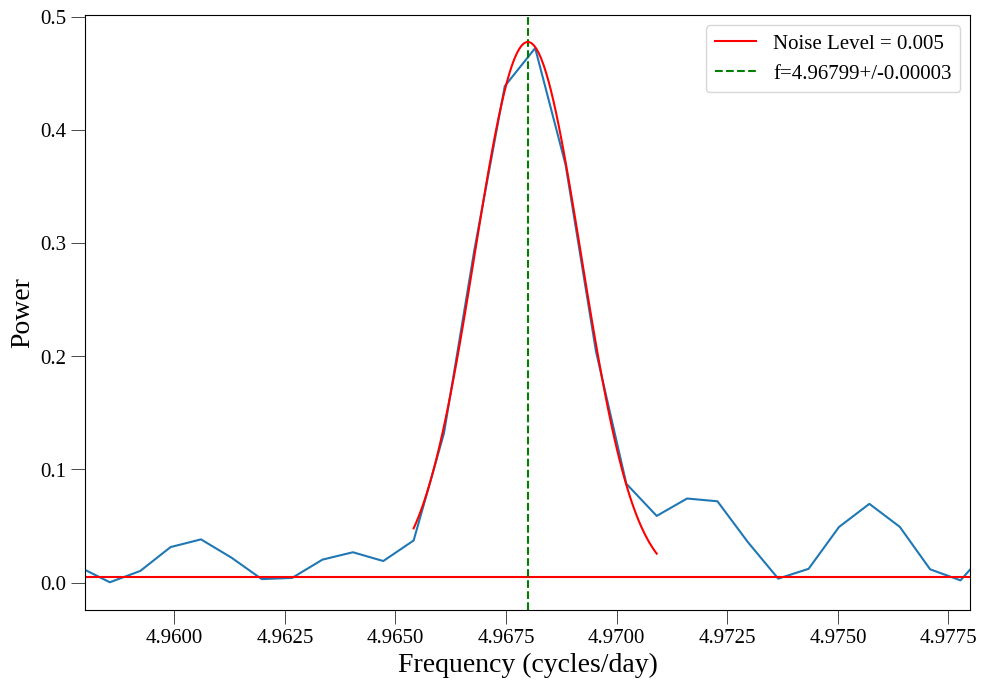
\includegraphics[width=0.5\textwidth]{1_ls_gaussian.png}
                \caption{Gaussovo fitování píku periodogramu pro dataset 1.dat.}
                \label{fig:1_ls_gaussian}
            \end{figure}
            
            K výpočtu veličin a jejich nejistot byla použita knihovna Uncertinties pro Python. Chyby byly rozšířeny o Studentův koeficient (2-Tail Confidence Level) s ohledem na stupně volnosti pro každou hodnotu, pro interval spolehlivosti 68.27\%.

    \section{Vysledky}
        \subsection{Původní soubory dat}
            Světelné křivky pro soubory dat 1, 2, 3, 4, 5 a 6 jsou zobrazeny na obrázcích (\ref{fig:1_ls}), (\ref{fig:2_ls}), (\ref{fig:3_ls}), (\ref{fig:4_ls}), (\ref{fig:5_ls}) a (\ref{fig:6_ls}) resp. Jejich odpovídající periodogramy jsou znázorněny na obrázcích (\ref{fig:1_per}), (\ref{fig:2_per}), (\ref{fig:3_per}), (\ref{fig:4_per}), (\ref{fig:5_per}) a (\ref{fig:6_per}). Frekvence, periody, síla, SNR a FAP jsou uvedeny v tabulkách (\ref{tab:1}), (\ref{tab:2}), (\ref{tab:3}), (\ref{tab:4}), (\ref{tab:5}) a (\ref{tab:6}).

            \begin{table}[htbp]
                \centering
                \vspace{-0.5em}
                \resizebox{\columnwidth}{!}{%
                    \pgfplotstabletypeset[
                        col sep=comma,
                        string type,
                        every head row/.style={before row=\toprule, after row=\midrule},
                        every last row/.style={after row=\bottomrule},
                        columns/frequency/.style={column name=Frequency [c/d]},
                        columns/period/.style={column name=Period [d]},
                        columns/power/.style={column name=Power},
                        columns/SNR/.style={column name=SNR},
                        columns/FAP/.style={column name=FAP},
                    ]{output/1.csv}
                }
                \caption{Vysledky analýzy pro dataset 1.dat.}
                \label{tab:1}
            \end{table}
            
            \begin{table}[htbp]
                \centering
                \vspace{-0.5em}
                \resizebox{\columnwidth}{!}{%
                    \pgfplotstabletypeset[
                        col sep=comma,
                        string type,
                        every head row/.style={before row=\toprule, after row=\midrule},
                        every last row/.style={after row=\bottomrule},
                        columns/frequency/.style={column name=Frequency [c/d]},
                        columns/period/.style={column name=Period [d]},
                        columns/power/.style={column name=Power},
                        columns/SNR/.style={column name=SNR},
                        columns/FAP/.style={column name=FAP},
                    ]{output/2.csv}
                }
                \caption{Vysledky analýzy pro dataset 2.dat.}
                \label{tab:2}
            \end{table}

            \begin{table}[htbp]
                \centering
                \vspace{-0.5em}
                \resizebox{\columnwidth}{!}{%
                    \pgfplotstabletypeset[
                        col sep=comma,
                        string type,
                        every head row/.style={before row=\toprule, after row=\midrule},
                        every last row/.style={after row=\bottomrule},
                        columns/frequency/.style={column name=Frequency [c/d]},
                        columns/period/.style={column name=Period [d]},
                        columns/power/.style={column name=Power},
                        columns/SNR/.style={column name=SNR},
                        columns/FAP/.style={column name=FAP},
                    ]{output/3.csv}
                }
                \caption{Vysledky analýzy pro dataset 3.dat.}
                \label{tab:3}
            \end{table}

            \begin{table}[htbp]
                \centering
                \vspace{-0.5em}
                \resizebox{\columnwidth}{!}{%
                    \pgfplotstabletypeset[
                        col sep=comma,
                        string type,
                        every head row/.style={before row=\toprule, after row=\midrule},
                        every last row/.style={after row=\bottomrule},
                        columns/frequency/.style={column name=Frequency [c/d]},
                        columns/period/.style={column name=Period [d]},
                        columns/power/.style={column name=Power},
                        columns/SNR/.style={column name=SNR},
                        columns/FAP/.style={column name=FAP},
                    ]{output/4.csv}
                }
                \caption{Vysledky analýzy pro dataset 4.dat.}
                \label{tab:4}
            \end{table}

            \begin{table}[htbp]
                \centering
                \vspace{-0.5em}
                \resizebox{\columnwidth}{!}{%
                    \pgfplotstabletypeset[
                        col sep=comma,
                        string type,
                        every head row/.style={before row=\toprule, after row=\midrule},
                        every last row/.style={after row=\bottomrule},
                        columns/frequency/.style={column name=Frequency [c/d]},
                        columns/period/.style={column name=Period [d]},
                        columns/power/.style={column name=Power},
                        columns/SNR/.style={column name=SNR},
                        columns/FAP/.style={column name=FAP},
                    ]{output/5.csv}
                }
                \caption{Vysledky analýzy pro dataset 5.dat.}
                \label{tab:5}
            \end{table}

            \begin{table}[htbp]
                \centering
                \vspace{-0.5em}
                \resizebox{\columnwidth}{!}{%
                    \pgfplotstabletypeset[
                        col sep=comma,
                        string type,
                        every head row/.style={before row=\toprule, after row=\midrule},
                        every last row/.style={after row=\bottomrule},
                        columns/frequency/.style={column name=Frequency [c/d]},
                        columns/period/.style={column name=Period [d]},
                        columns/power/.style={column name=Power},
                        columns/SNR/.style={column name=SNR},
                        columns/FAP/.style={column name=FAP},
                    ]{output/6.csv}
                }
                \caption{Vysledky analýzy pro dataset 6.dat.}
                \label{tab:6}
            \end{table}

            \begin{figure*}%[htbp]
                \centering
                \begin{subfigure}[t]{0.48\textwidth}
                    \centering
                    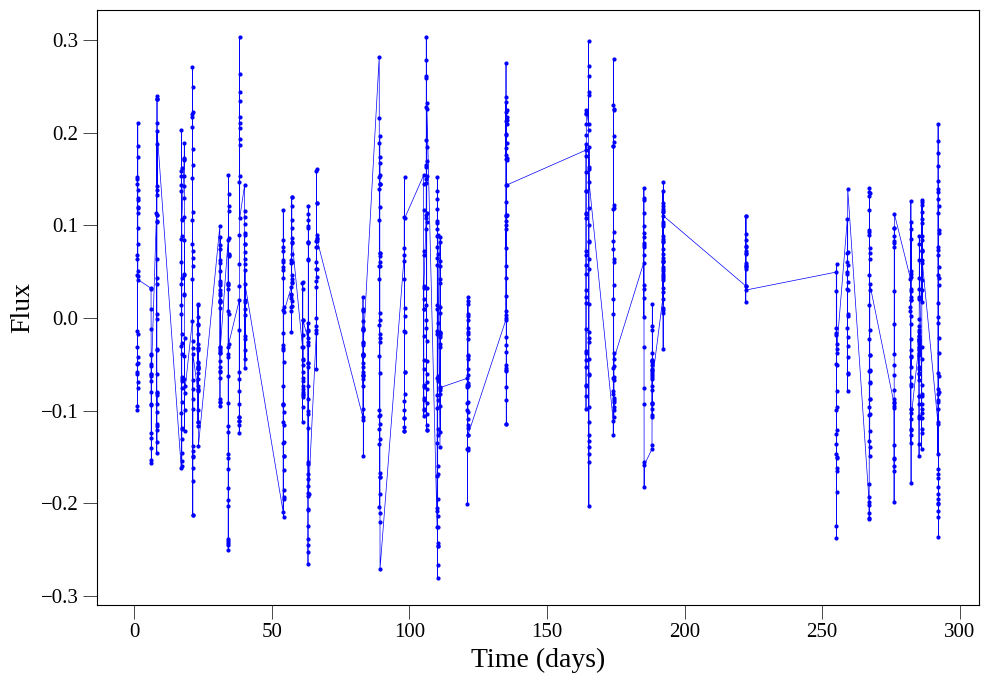
\includegraphics[width=\textwidth]{1_ls.png}
                    \caption{Světelná křivka pro dataset 1.dat.}
                    \label{fig:1_ls}
                \end{subfigure}
                \hfill
                \begin{subfigure}[t]{0.48\textwidth}
                    \centering
                    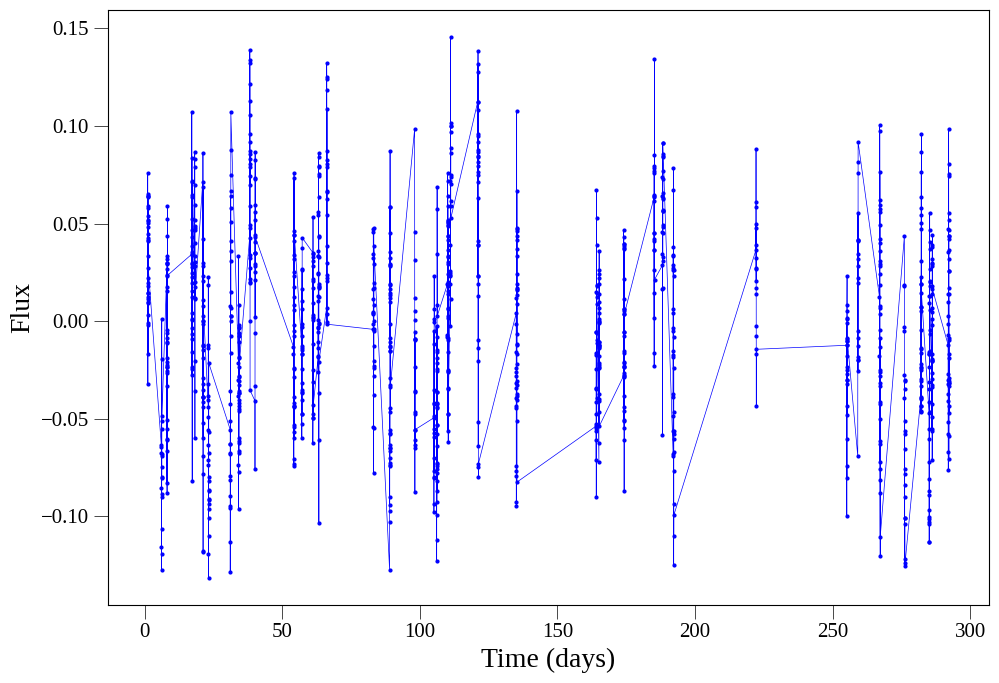
\includegraphics[width=\textwidth]{2_ls.png}
                    \caption{Světelná křivka pro dataset 2.dat.}
                    \label{fig:2_ls}
                \end{subfigure}
                \hfill
                \begin{subfigure}[t]{0.48\textwidth}
                    \centering
                    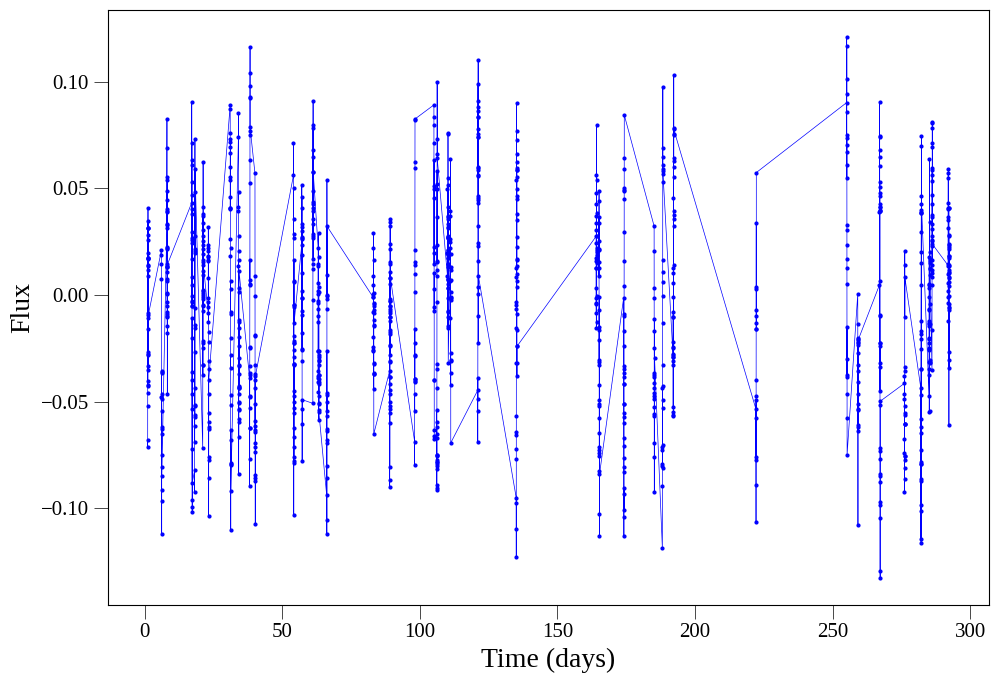
\includegraphics[width=\textwidth]{3_ls.png}
                    \caption{Světelná křivka pro dataset 3.dat.}
                    \label{fig:3_ls}
                \end{subfigure}
                \vspace{10pt}
                \begin{subfigure}[t]{0.48\textwidth}
                    \centering
                    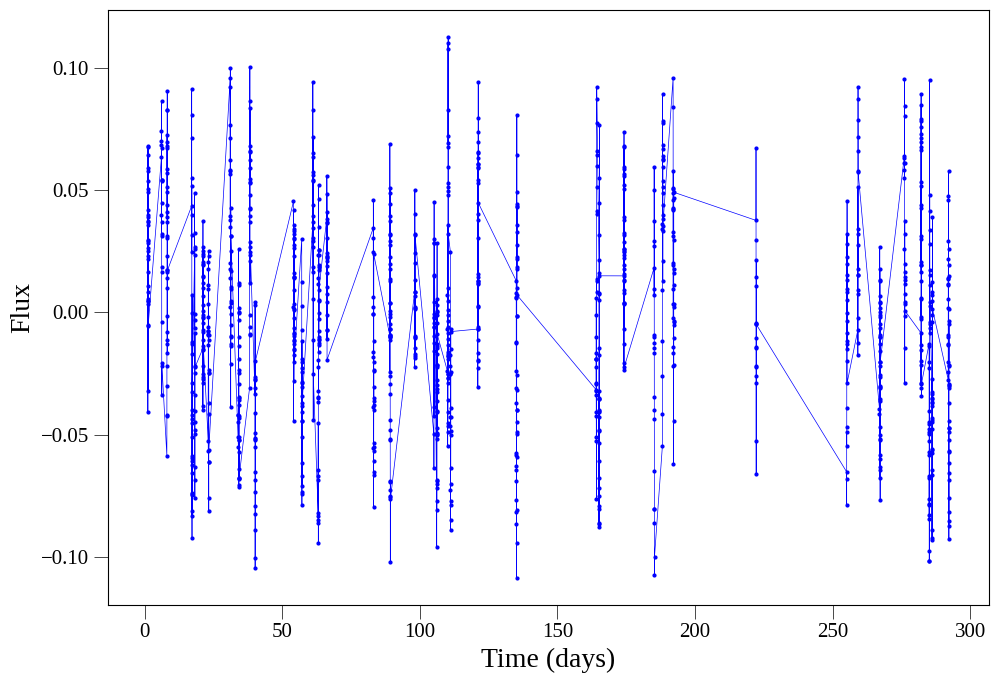
\includegraphics[width=\textwidth]{4_ls.png}
                    \caption{Světelná křivka pro dataset 4.dat.}
                    \label{fig:4_ls}
                \end{subfigure}
                \hfill
                \begin{subfigure}[t]{0.48\textwidth}
                    \centering
                    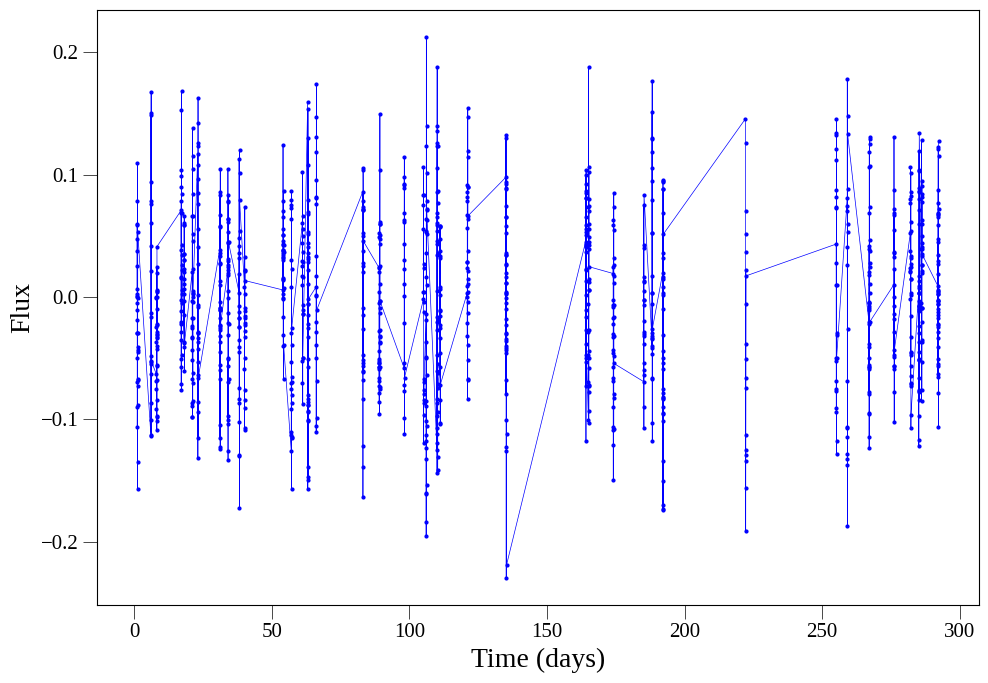
\includegraphics[width=\textwidth]{5_ls.png}
                    \caption{Světelná křivka pro dataset 5.dat.}
                    \label{fig:5_ls}
                \end{subfigure}
                \hfill
                \begin{subfigure}[t]{0.48\textwidth}
                    \centering
                    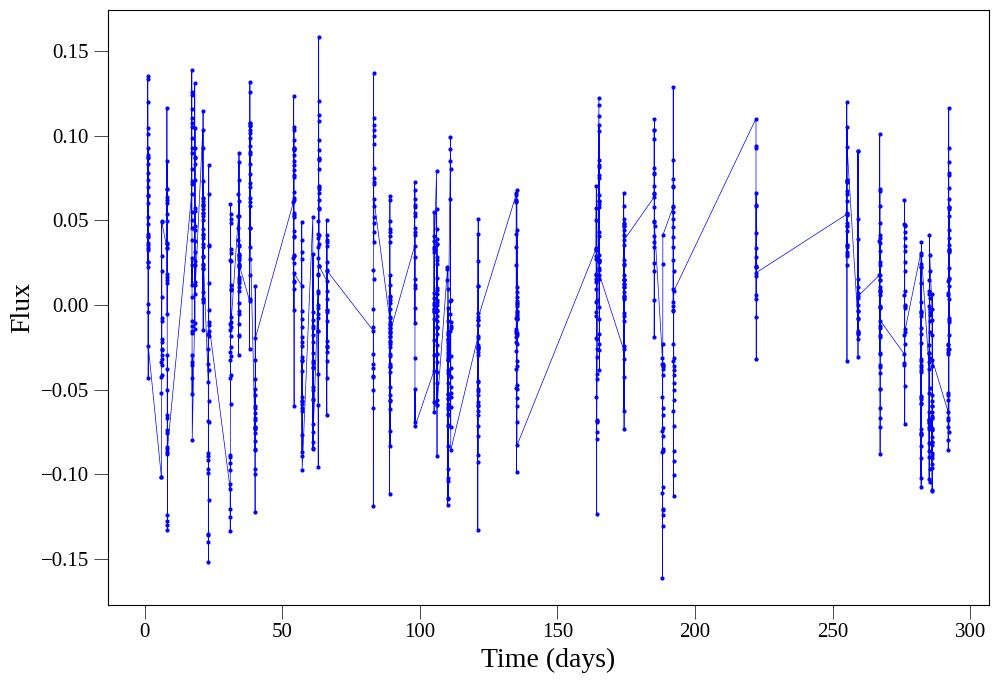
\includegraphics[width=\textwidth]{6_ls.png}
                    \caption{Světelná křivka pro dataset 6.dat.}
                    \label{fig:6_ls}
                \end{subfigure}
                \caption{Světelné křivky pro všechny datasety.}
                \label{fig:all_lc}
            \end{figure*}

            \begin{figure*}%[htbp]
                \centering
                \begin{subfigure}[t]{0.48\textwidth}
                    \centering
                    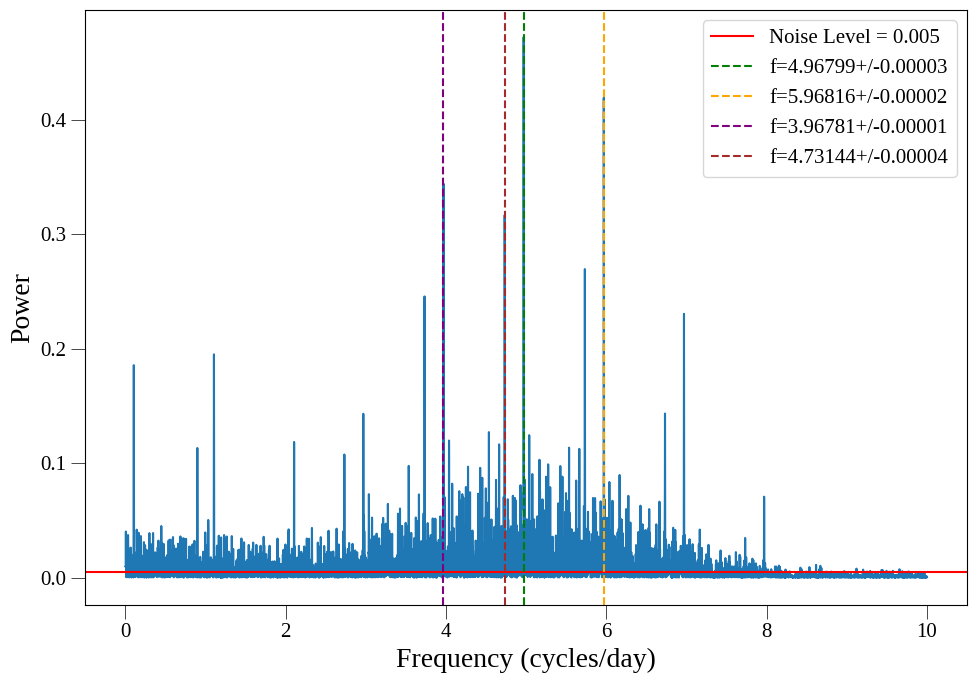
\includegraphics[width=\textwidth]{1_per.png}
                    \caption{Periodogram pro dataset 1.dat.}
                    \label{fig:1_per}
                \end{subfigure}
                \hfill
                \begin{subfigure}[t]{0.48\textwidth}
                    \centering
                    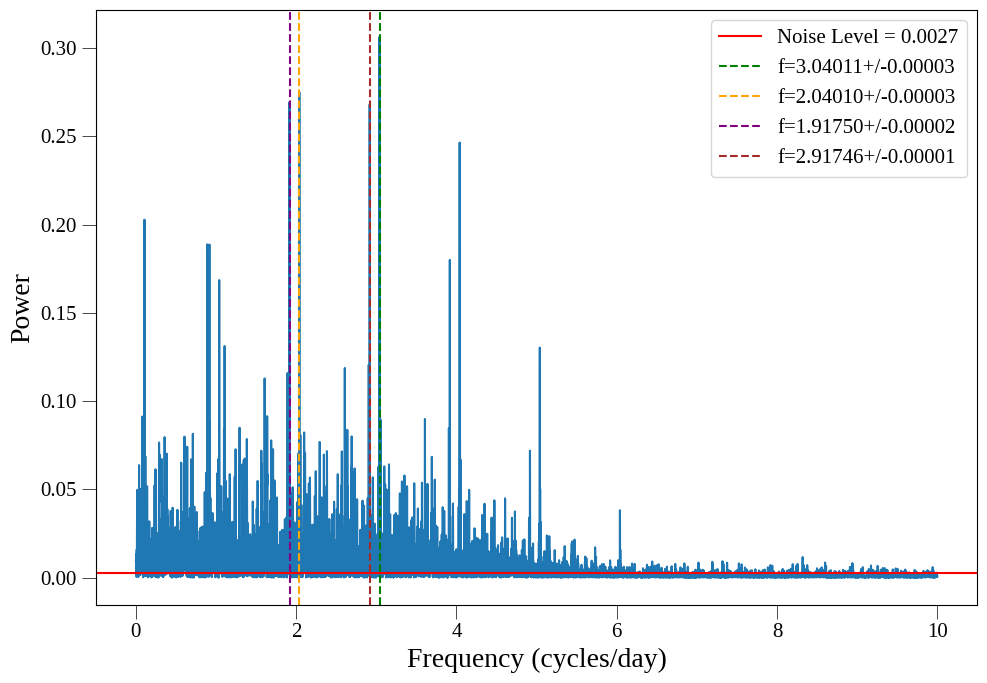
\includegraphics[width=\textwidth]{2_per.png}
                    \caption{Periodogram pro dataset 2.dat.}
                    \label{fig:2_per}
                \end{subfigure}
                \hfill
                \begin{subfigure}[t]{0.48\textwidth}
                    \centering
                    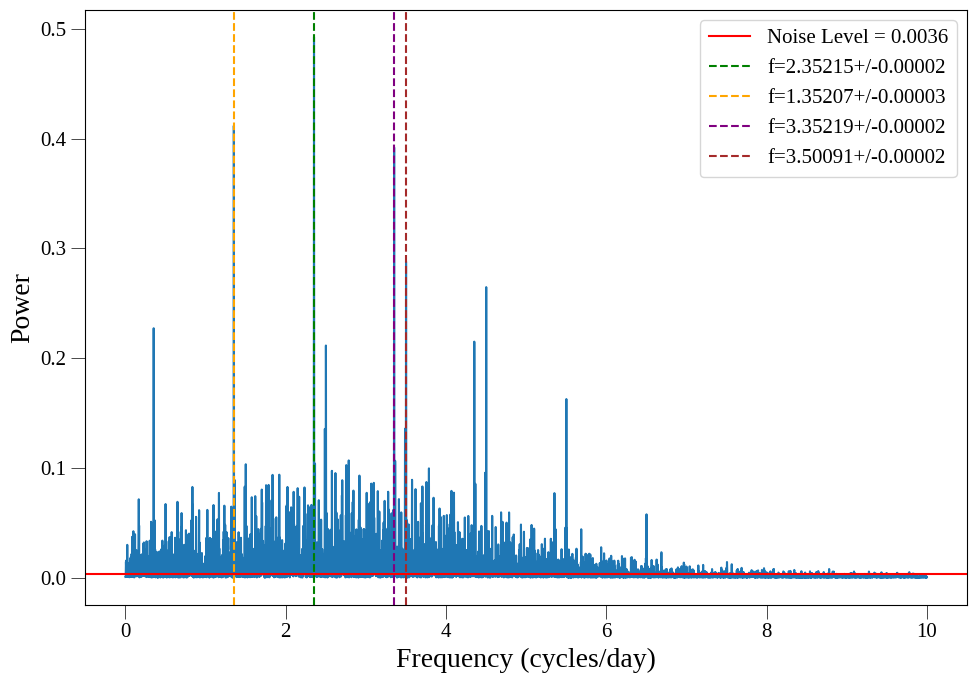
\includegraphics[width=\textwidth]{3_per.png}
                    \caption{Periodogram pro dataset 3.dat.}
                    \label{fig:3_per}
                \end{subfigure}
                \vspace{10pt}
                \begin{subfigure}[t]{0.48\textwidth}
                    \centering
                    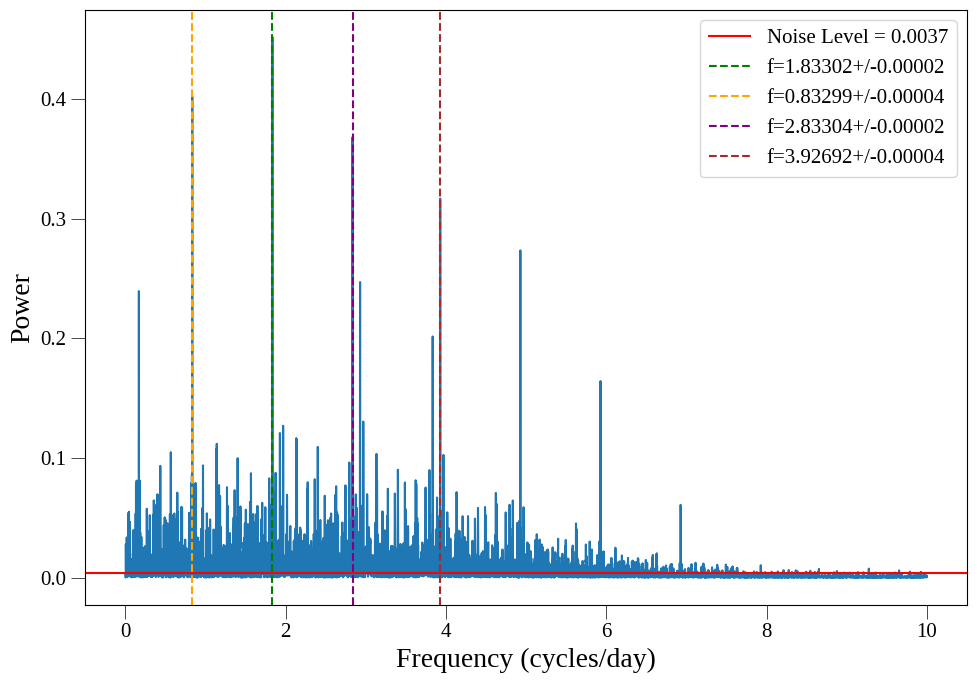
\includegraphics[width=\textwidth]{4_per.png}
                    \caption{Periodogram pro dataset 4.dat.}
                    \label{fig:4_per}
                \end{subfigure}
                \hfill
                \begin{subfigure}[t]{0.48\textwidth}
                    \centering
                    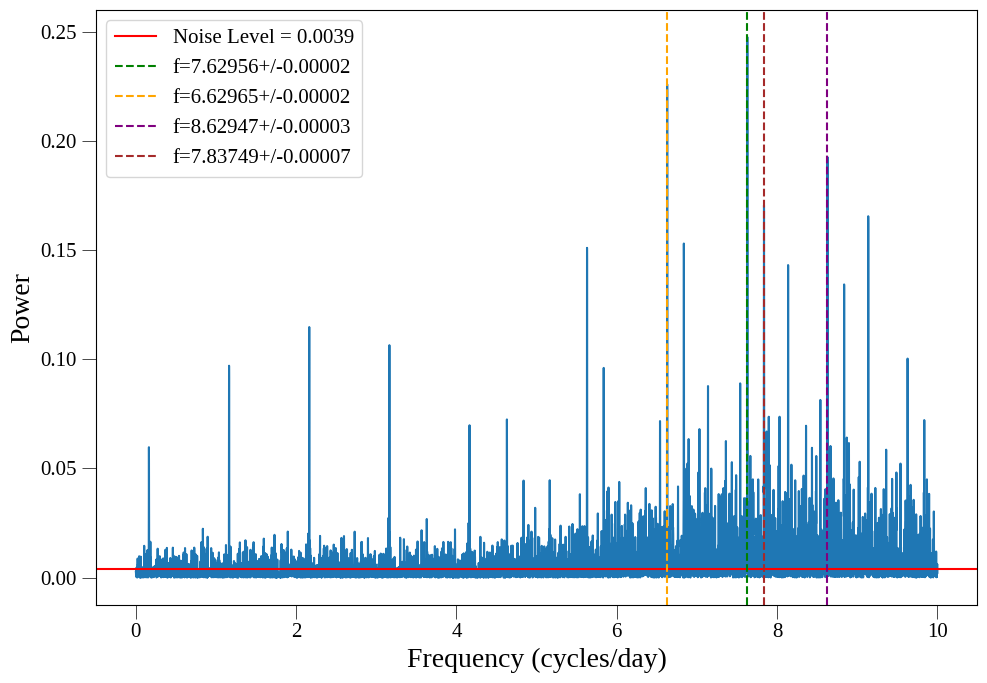
\includegraphics[width=\textwidth]{5_per.png}
                    \caption{Periodogram pro dataset 5.dat.}
                    \label{fig:5_per}
                \end{subfigure}
                \hfill
                \begin{subfigure}[t]{0.48\textwidth}
                    \centering
                    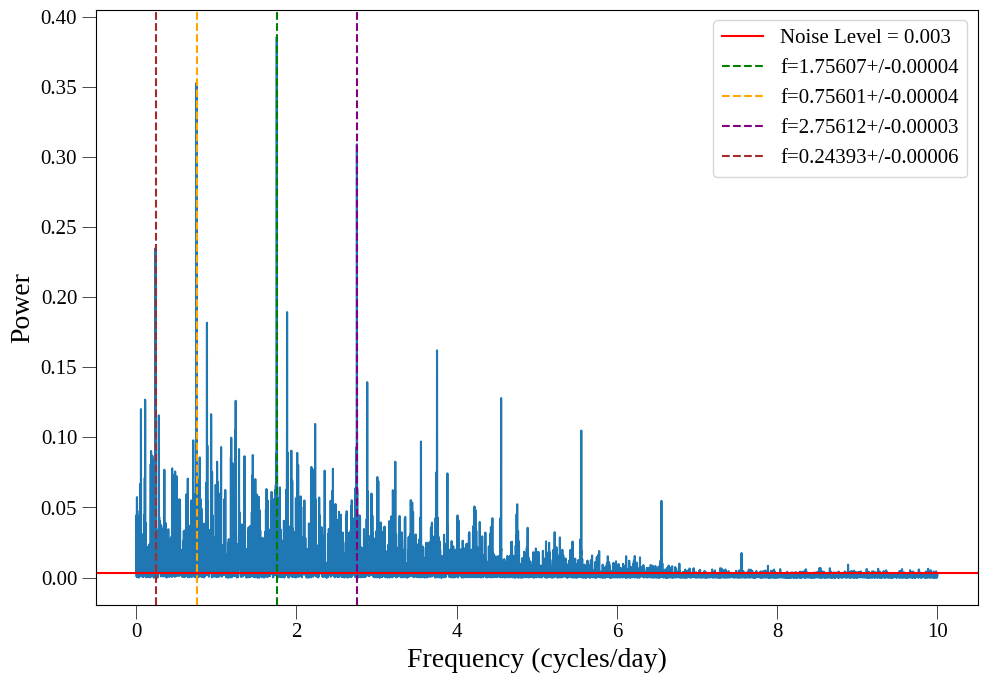
\includegraphics[width=\textwidth]{6_per.png}
                    \caption{Periodogram pro dataset 6.dat.}
                    \label{fig:6_per}
                \end{subfigure}
                \caption{Periodogramy pro všechny datasety.}
                \label{fig:all_per}
            \end{figure*}

        \newpage
        \subsection{Kepler-22}
            Světelná křivka pro Kepler-22 je zobrazena na obrázku (\ref{fig:kplr_ls}). Odpovídající periodogram je znázorněn na obrázku (\ref{fig:kplr_per}). Frekvence, periody, síla, SNR a FAP pro Kepler-22 jsou uvedeny v tabulce (\ref{tab:kplr}).

            \begin{table}[htbp]
                \centering
                \resizebox{\columnwidth}{!}{%
                    \pgfplotstabletypeset[
                        col sep=comma,
                        string type,
                        every head row/.style={before row=\toprule, after row=\midrule},
                        every last row/.style={after row=\bottomrule},
                        columns/frequency/.style={column name=Frequency [c/d]},
                        columns/period/.style={column name=Period [d]},
                        columns/power/.style={column name=Power},
                        columns/SNR/.style={column name=SNR},
                        columns/FAP/.style={column name=FAP},
                    ]{output/kplr.csv}
                }
                \caption{Vysledky analýzy pro Kepler-22.}
                \label{tab:kplr}
            \end{table}

            \begin{figure}
                \centering
                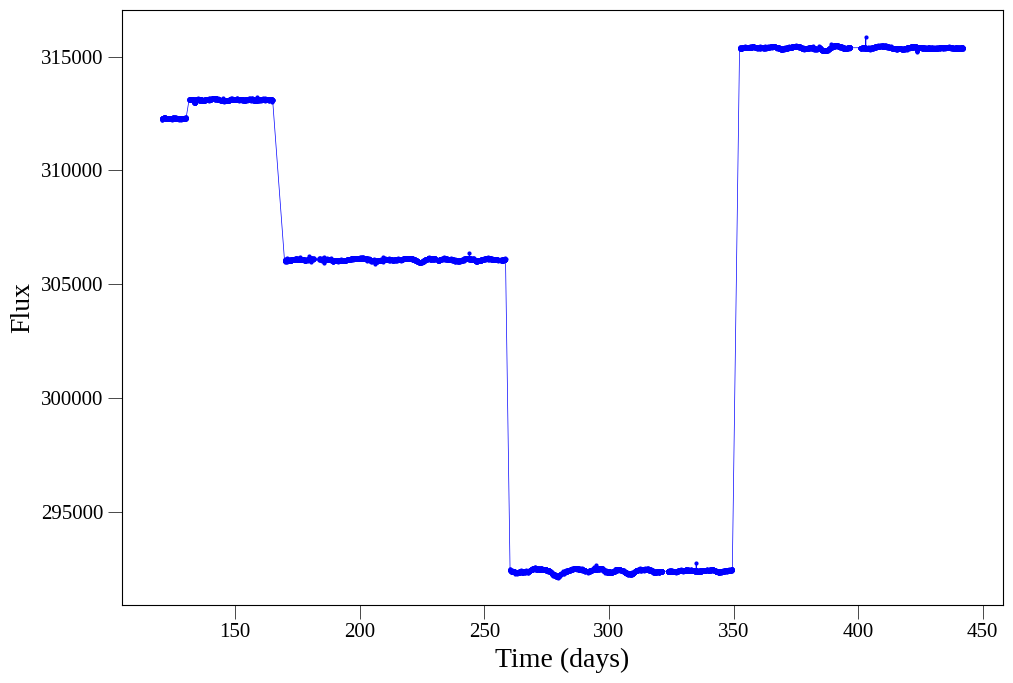
\includegraphics[width=0.5\textwidth]{kplr_ls.png}
                \caption{Světelná křivka pro Kepler-22.}
                \label{fig:kplr_ls}
            \end{figure}

            \begin{figure}
                \centering
                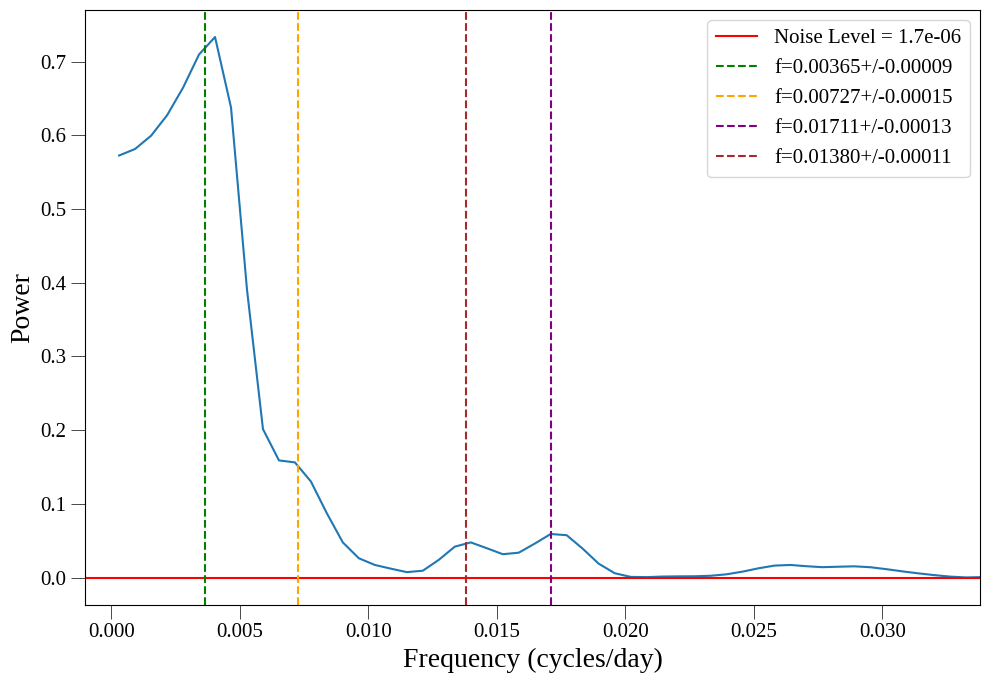
\includegraphics[width=0.5\textwidth]{kplr_per.png}
                \caption{Periodogram pro Kepler-22.}
                \label{fig:kplr_per}
            \end{figure}
    
    \newpage
    \section{Závěr}
        Analýzy periodogramů pro soubory dat 1, 2, 3, 4, 5 a 6 ukazují, že všechny nalezené signifikantní frekvence jsou spolehlivé, protože mají vysoký SNR a nízký FAP. Vzhledem k jednotlivým periodám lze předpokládat, že obecně jsou pro periodickou aktivitu způsobenou planetami periody poměrně malé. Nejpravděpodobnější povahou periodicity je tedy proměnlivost samotné hvězdy. 

        Některé periody (např. periody datových sad 2, 3, 4 a 6) však mohou naznačovat možnou přítomnost exoplanet s ultrakrátkými periodami (viz. \citet{frustagli2020} a \citet{wang2024}). Periody datových sad 4 a 6 ($\text{P} = 1.20049(6) ~ \text{d}$ a $\text{P} = 1.32273(8) ~ \text{d}$) naznačují možnou přítomnost exoplanet s krátkými periodami. Obě však vyžadují další, sofistikovanější analýzy. 
        
        Výsledky analýzy periodogramu pro Kepler-22 ukazují, že signifikantní frekvence odpovídají periodám, které by mohly být způsobeny oběžnými pohyby exoplanet. Výsledky jsou v souladu s předchozími studiemi, které naznačují, že Kepler-22 ma znamou exoplanetu Kepler-22b s periodou $\text{P} = 289.8623(2) ~ \text{d}$ (viz. \citet{borucki2012}). Dostal jsem hodnotu $\text{P} = 234(7) ~ \text{d}$, což je v souladu s literaturou.
    % \newpage

    \bibliographystyle{plainnat}
    \bibliography{refs/bibliography}

\end{document}